\documentclass[tikz,border=3pt]{standalone}
\usepackage[T1]{fontenc}
\usepackage{amsmath}
\usepackage{XCharter}
\usepackage[xcharter]{newtxmath}
\usepackage[scaled=.92]{helvet}
\usepackage{pgfplots}
\usetikzlibrary{arrows.meta,positioning,fit,calc,backgrounds,decorations.pathreplacing,patterns}
\usepgfplotslibrary{groupplots,fillbetween}
\pgfplotsset{compat=1.18}
\definecolor{ink}{HTML}{172536}
\definecolor{rgb}{HTML}{3563B8}
\definecolor{event}{HTML}{17857C}
\definecolor{fusion}{HTML}{76529C}
\definecolor{reference}{HTML}{8994A3}
\definecolor{warn}{HTML}{AC5948}
\definecolor{muted}{HTML}{657183}
\definecolor{rule}{HTML}{D9E0E8}
\definecolor{pale}{HTML}{F5F7FA}
\color{ink}
\tikzset{box/.style={rounded corners=2pt,draw=rule,fill=white,align=center,inner sep=4pt,font=\sffamily\fontsize{9}{10.8}\selectfont,minimum height=9mm},rb/.style={box,draw=rgb!50,fill=rgb!5},eb/.style={box,draw=event!50,fill=event!5},fb/.style={box,draw=fusion!55,fill=fusion!5},arrow/.style={-{Latex[length=1.8mm]},line width=.65pt,draw=muted},note/.style={font=\sffamily\fontsize{8.4}{10.2}\selectfont,align=center,text=muted},heading/.style={font=\sffamily\fontsize{10}{12}\selectfont\bfseries,align=left,text=ink}}
\pgfplotsset{paper/.style={width=15.7cm,height=6cm,axis lines*=left,axis line style={rule},tick style={draw=none},tick label style={font=\sffamily\fontsize{8.8}{10.4}\selectfont,text=muted},label style={font=\sffamily\fontsize{9.4}{11}\selectfont,text=ink},title style={font=\sffamily\fontsize{10}{12}\selectfont\bfseries,text=ink},legend style={draw=none,fill=none,font=\sffamily\fontsize{9}{11}\selectfont,cells={anchor=west}},grid=major,grid style={rule!65,line width=.3pt},minor tick num=0,scaled ticks=false,unbounded coords=jump,clip mode=individual}}
\begin{document}

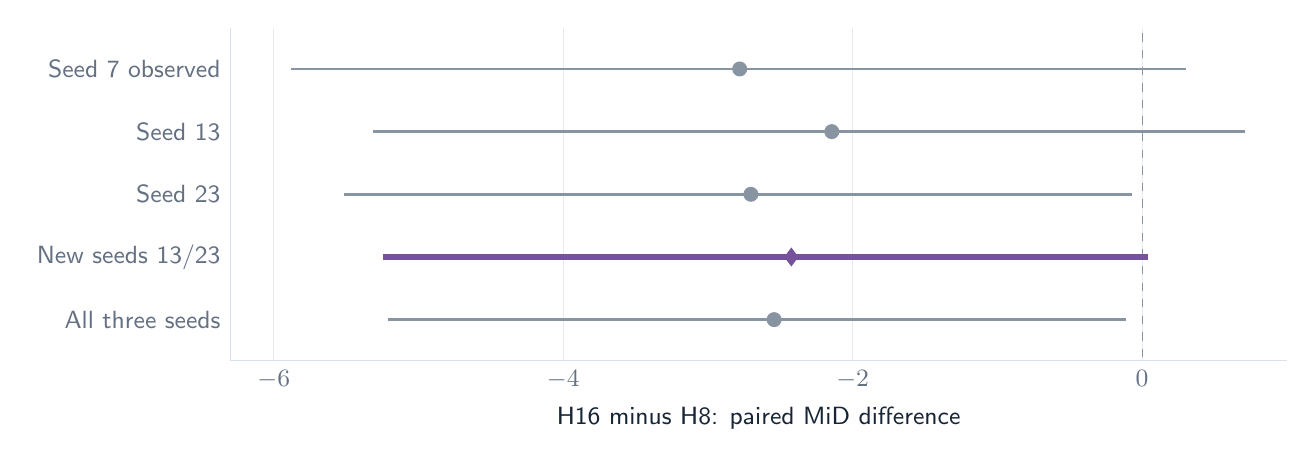
\begin{tikzpicture}
\begin{axis}[paper,width=15.0cm,height=5.8cm,xmin=-6.3,xmax=1,ymin=-.65,ymax=4.65,ytick={0,1,2,3,4},yticklabels={All three seeds,New seeds 13/23,Seed 23,Seed 13,Seed 7 observed},xlabel={H16 minus H8: paired MiD difference},xtick={-6,-4,-2,0},ymajorgrids=false]
\draw[dashed,reference] (axis cs:0,-.6)--(axis cs:0,4.6);
\addplot[reference,line width=1pt] coordinates {(-5.87938910434867,4) (0.301408689883551,4)};
\addplot[reference,line width=1pt] coordinates {(-5.31728177927018,3) (0.711787178409021,3)};
\addplot[reference,line width=1pt] coordinates {(-5.51443214969556,2) (-0.0705419668049701,2)};
\addplot[fusion,line width=1.9pt] coordinates {(-5.24425945475314,1) (0.0410914851845699,1)};
\addplot[reference,line width=1pt] coordinates {(-5.21339788936392,0) (-0.111240531080439,0)};
\addplot[only marks,mark=*,reference,mark size=2.5pt] coordinates {(-2.78059334730865,4) (-2.144150258867,3) (-2.70325429323855,2) (-2.5426659664714,0)};
\addplot[only marks,mark=diamond*,fusion,mark size=3.1pt] coordinates {(-2.42370227605277,1)};
\end{axis}\end{tikzpicture}
\end{document}
